%!TEX root = ../thesis.tex
\begin{savequote}[75mm]
If a team couldn’t be fed with two pizzas, it was too big.
\qauthor{Jeff Bezos}
\end{savequote}

% https://areomagazine.com/2019/04/10/agile-and-the-software-industrys-ideology-problem/ 
%https://www.softwaretestinghelp.com/agile-manifesto/
%http://www.ambysoft.com/essays/agileManifesto.html
%https://www.smartsheet.com/comprehensive-guide-values-principles-agile-manifesto

\chapter{Agile Software Development}

Before getting into the implementation and adaptation of Jira and Confluence, let's back up a little and understand the concept of Agile, a Software Development Life Cycle (or SDLC) model.

SDLCs did not emerge until the 1960s, they are considered to be the oldest formalization of framework.
%The Space Shuttle program, which operationally launched in 1982, used information and processing technologies from the 1960s.
%https://ase.in.tum.de/paid.globalse.org/paid1/courseDocs/Readings/SoftwareLifeCycle030398.pdf
A SDLC refers to the ensemble of activities that compose a software project.
It starts with the concepts of understanding the problem and the requirements and it ends with the retirement of the system (when there is no more maintenance) or with the cancellation of the project.

Small projects (generally for a single person) have a simpler life cycle: find the problem and write a program to solve it.
Once the problem has been solved, the program can be deleted and forgotten.

%todo or in larger problems / solved
In larger projects, that require a team to be developed, there must be some explicit rules to set a higher quality of the software.
As activities are assigned to different persons, it becomes critical that all participants share a common view of the execution of the project.
A SDLC model is a framework providing the ordering and dependencies of life cycle activities. 

%todo rivedere
Managing dependencies among other activities can be a major impact for a successful project and its duration. 
For example, a change in requirements during implementation may invalidate a substantial amount of work and delay the delivery of the system by several months.
Different life cycle models prescribe different actions to handle such changes.

%https://en.wikipedia.org/wiki/Software_development_process
There are many SDLCs like Waterfall, Prototyping, Iterative and Incremental Development, Spiral Development, Rapid Application Development, and Extreme Programming. (XP). 

%todo modificare immagine
\begin{figure}[H]
	\centering
	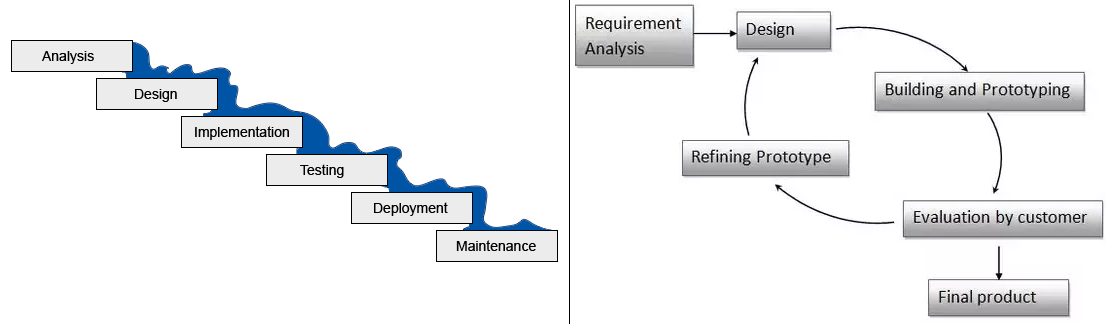
\includegraphics[width=\textwidth]{resources/warterfall_prototype}\\
	\caption{The Waterfall and Prototype SDLC models}
\end{figure}

%https://www.iso.org/obp/ui/#iso:std:iso-iec:tr:24774:ed-2:v1:en
%todo citare https://www.iso.org/standard/53815.html !!
As the word model suggests, each company may have its own SDLC designed ad hoc for their internal use.
This led to the creation of a standard that presents the guidelines for the elements that are most frequently used in describing a process: the title, purpose, outcomes, activities, task and information item.
The ISO/IEC TR 24774:2010: Systems and software engineering -- Life cycle management -- Guidelines for process description. %todo citare

The complexity and slowness in producing a concrete product in older SDLCs brought the need for a faster and more communicative model.

%https://www.tutorialspoint.com/sdlc/sdlc_agile_model.htm
%todo mettere a glossario
%Agile SDLC model is a combination of iterative and incremental process models with focus on process adaptability and customer satisfaction by rapidly and continuously deliver of working software product.

This chapter describes the most fundamental points of the Agile method, how it started and the adaptations that derived from it, like Scrum.
At the end, it also explains how Athonet's adaptation of the Agile life cycle works.

\begin{figure}[H]
	\centering
	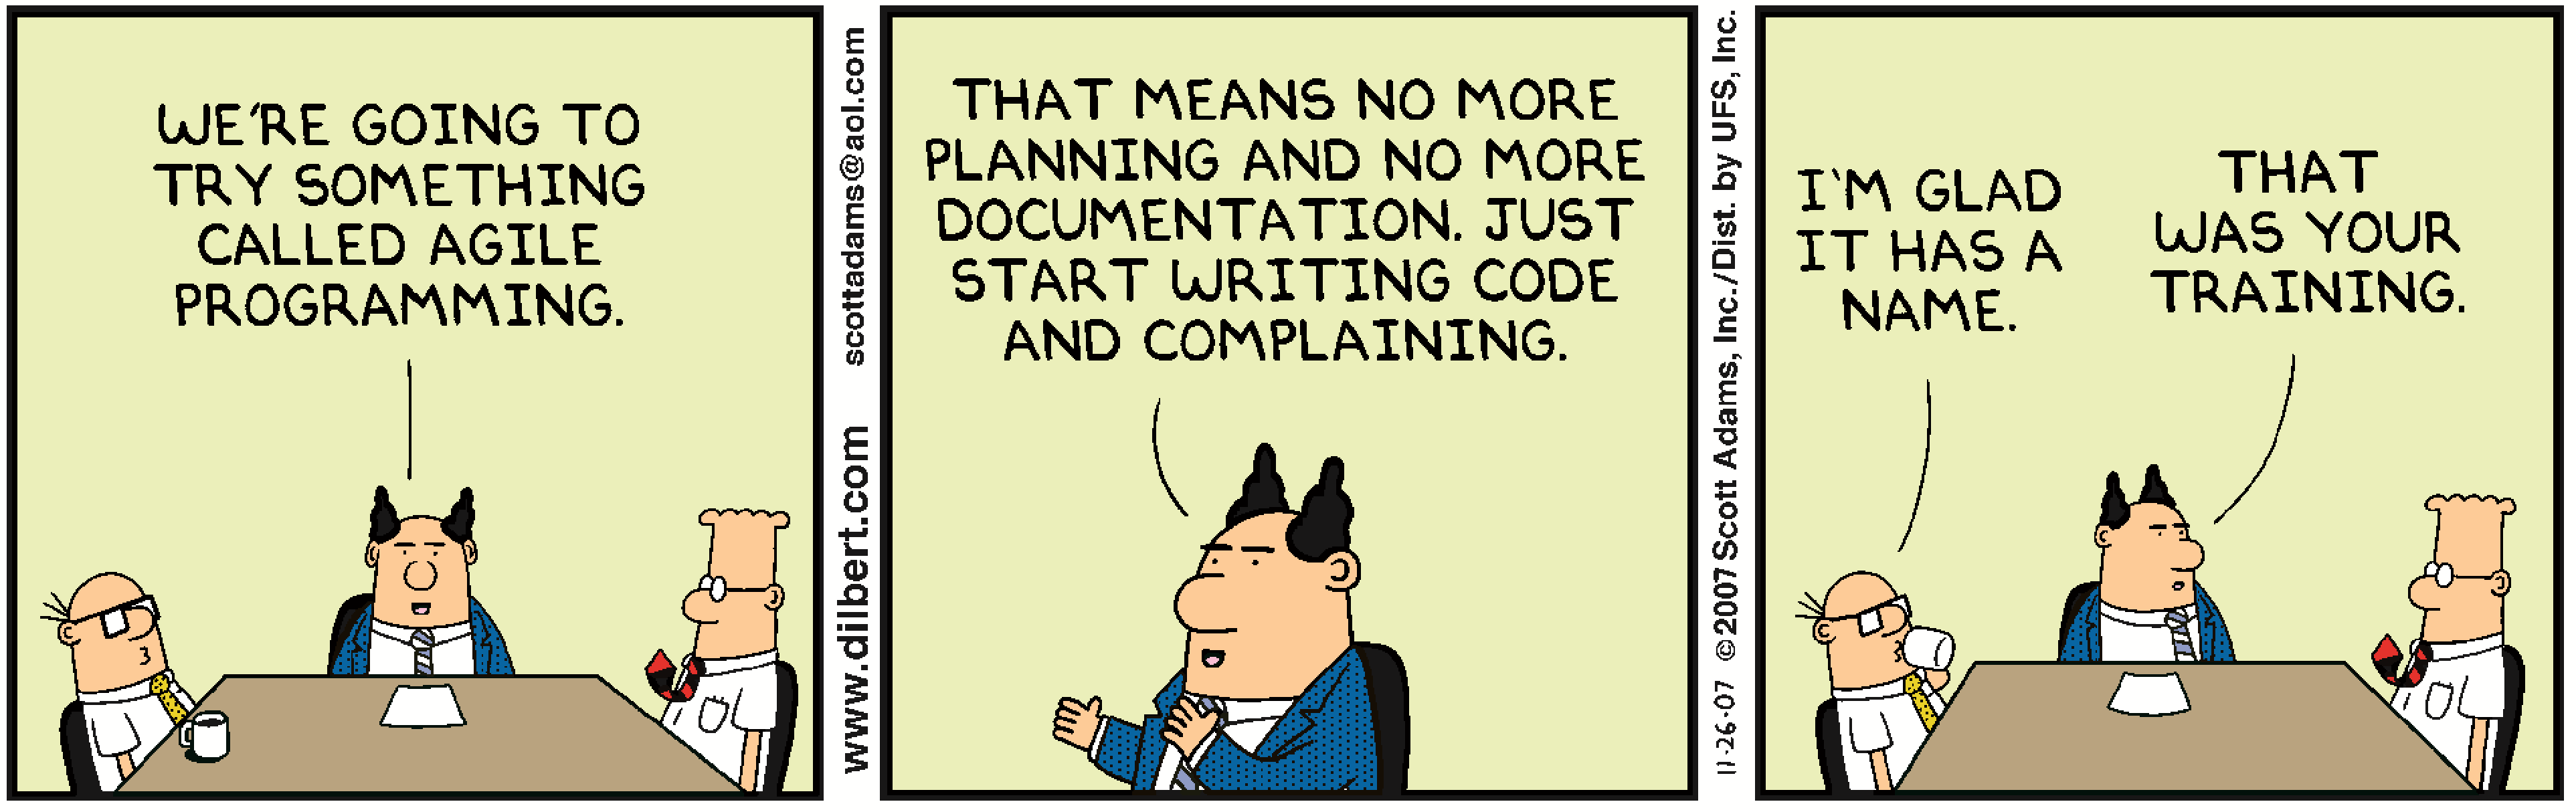
\includegraphics[width=\textwidth]{resources/Dilbert_Training_Agile_Programming}\\
	\caption{Dilbert on Agile Programming}
\end{figure}

%https://techbeacon.com/app-dev-testing/agility-beyond-history-legacy-agile-developmentdls
\section{Why the need for a new Software Life Cycle}

	The decade of 1990 represented a very important turning point for the digital industry.
	Computers were spreading everywhere and the software companies faced the so called application development crisis.
	
	The problem was that businesses moved too fast and within the space of three years, requirements, systems, and even entire businesses were likely to change. %todo citare sito
	
	It meant that a lot of software ended up being incomplete or canceled halfway and the ones that made it through, even if they fulfilled the original objectives of the client, may not meet all the business needs.

%	https://hackr.io/blog/sdlc-methodologies
	SDLC models can be of two types:
	\begin{itemize}
		\item Iterative: (like ..)
		\item Incremental: (like .. )
	\end{itemize}
	
	Two characteristic models used before Agile where the Sequential model (or Waterfall) and the Incremental model.

	%todo completare
	The pros / cons of waterfall were ... 
	The pros / cons of x where ...

	The excessive documentation, the forceful binding to the unchangeable decisions made early in the project and the little communication with the client brought to the need of a new model that prioritizes the product and the stakeholders over bureaucracy. 

	Those things frustrated people like Jon Kern, an aerospace engineer in the 1990s that with other figures from different industries "were looking for something that was more timely and responsive", as he noted.
	He was one of 17 software leaders that started meeting informally and talking about ways to develop software in a simpler way without the excess of documentation and other strict rules.

	These talks led to the now famous Snowbird meeting (in Utah, February 2001), when the Agile Manifesto was written down and published.

% https://agilemanifesto.org/
%https://www.productplan.com/glossary/agile-manifesto/
\section{The Agile manifesto}

	%todo inserire riferimento
	The Agile Manifesto is a brief document built on four foundational values and twelve supporting principles for Agile software development. 
%	The Agile Manifesto was published in February 2001 and is the work of 17 software development practitioners who observed the increasing need for an alternative to documentation-driven and heavyweight software development processes.

	%todo citare manifesto
	The four values are:
	\begin{itemize}
		\item \textbf{Individuals and interactions} over processes and tools
		\item \textbf{Working software} over comprehensive documentation
		\item \textbf{Customer collaboration} over contract negotiation
		\item \textbf{Responding to change} over following a plan
	\end{itemize}

	The responsiveness of people and embracing the importance of changes are the fundamentals of Agile.
	Although documentation is secondary, it's important to note that Agile streamlines documentation and does not eliminate it.

	These twelve principles emphasize things like “early and continuous delivery of valuable software” and “continuous attention to technical excellence”, and are: %todo citare manifesto
	\begin{enumerate}
		\item Our highest priority is to satisfy the customer through early and continuous delivery of valuable software.
		\item Welcome changing requirements, even late in development. Agile processes harness change for the customer's competitive advantage.
		\item Deliver working software frequently, from a couple of weeks to a couple of months, with a preference to the shorter timescale.
		\item Business people and developers must work together daily throughout the project.	
		\item Build projects around motivated individuals. Give them the environment and support they need, and trust them to get the job done.
		\item The most efficient and effective method of conveying information to and within a development team is face-to-face conversation.
		\item Working software is the primary measure of progress.
		\item Agile processes promote sustainable development. The sponsors, developers, and users should be able to maintain a constant pace indefinitely.	
		\item Continuous attention to technical excellence and good design enhances agility.
		\item Simplicity--the art of maximizing the amount of work not done--is essential.
		\item The best architectures, requirements, and designs emerge from self-organizing teams.
		\item At regular intervals, the team reflects on how to become more effective, then tunes and adjusts its behavior accordingly.
	\end{enumerate}
	
	All of them are important but, in my opinion, the ones that add the most value to the Agile line of thought and that differentiate it from the other methods are 2, 4 and 6.
	They represent the intent of placing the product and the customer above everything else, allowing the use of small informal meetings (even if the decisions should be recorded) and the easy change of requirements because the client is always involved, even as an end user (tester). 

	%https://medium.com/hygger-io/4-values-of-the-agile-manifesto-and-12-agile-principles-easily-explained-84cd429f69f
	Each Agile methodology applies the four values in different ways.
	However, all of them rely on these values to guide the development and delivery of high-quality, working software.

% Agile adaptations
\section{Agile's little big cousins}
	
	While Agile's manifesto contains values and principles, these are not prescriptive.
	In fact the manifesto does not outline specific processes, procedures or best practices.
	The goal is not to develop a rigid framework but rather create a mindset for software development.
	
	Agile is a blanket term that describes a set of software development principles.
	
	%	https://explore.versionone.com/state-of-agile
	There are many methodologies that derive from Agile's thinking, the most famous ones, according to the annual survey from VersionOne's team are:
	\begin{itemize}
		\item Scrum
		\item Scrumban
		\item Kanban
		\item Extreme Programming (XP)
	\end{itemize}

	\begin{figure}[H]
		\centering
		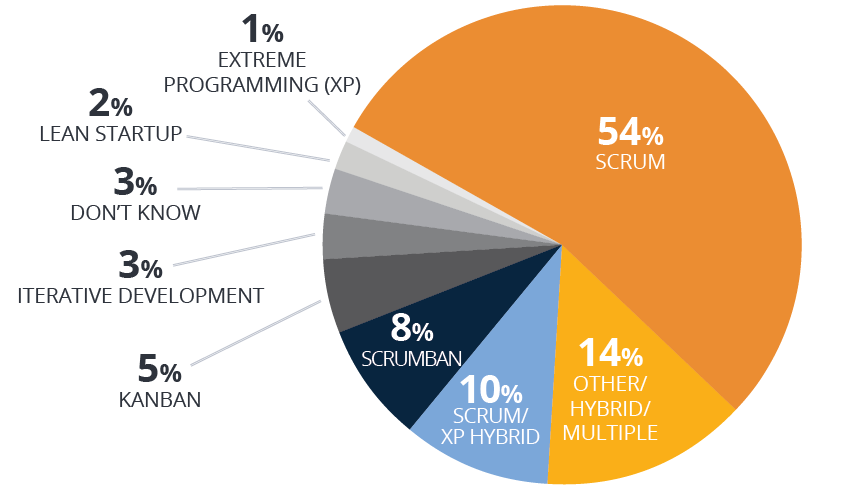
\includegraphics[width=.8\textwidth]{resources/agile-usage-chart}\\
		\caption{The Waterfall and Prototype SDLC models}
	\end{figure}

	%todo modificare immagine
	\begin{figure}[H]
		\centering
		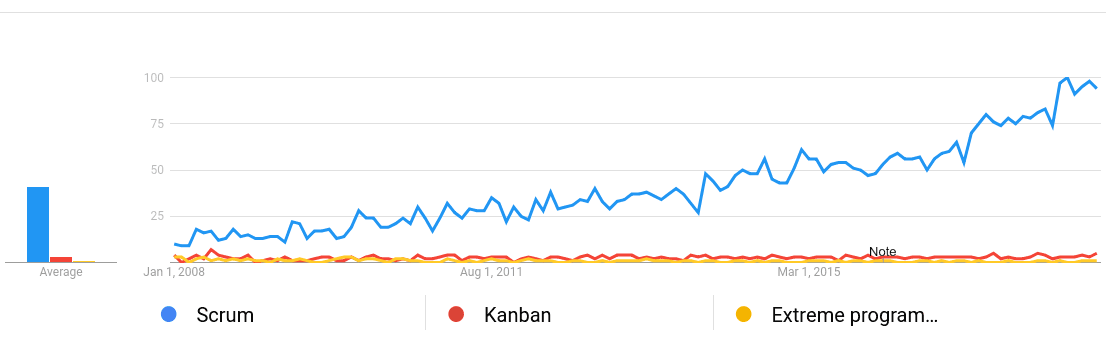
\includegraphics[width=\textwidth]{resources/trends}\\
		\caption{The Waterfall and Prototype SDLC models}
	\end{figure}
	
	This survey is quite interesting because it provides information from small and big real companies that want to share their experience.
	A very important fact to be noted is that although Technology companies are the ones that mostly participated to the survey, there are other industries that use Agile and are interested in sharing their experience.

	\begin{figure}[H]
		\centering
		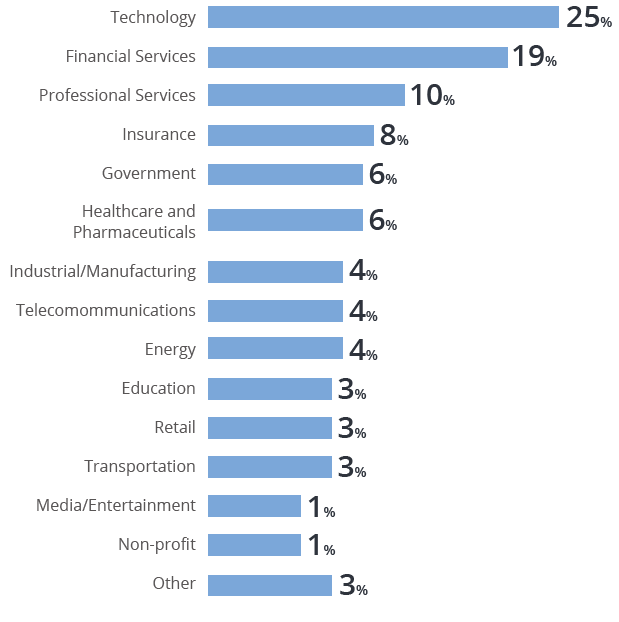
\includegraphics[width=.8\textwidth]{resources/Untitled_2}\\
		\caption{The Waterfall and Prototype SDLC models}
	\end{figure}

	It states that for the year 2018 (which marked their 13th annual report) the reasons for adopting Agile were productivity, improving team morale, reducing product risk (with a lesser percentage than the previous year) and about reducing project costs.

	The most cited measures of success cited by the respondents are customer, or user, satisfaction and business value.

	According to these companies, the benefits of adopting Agile are:
	\begin{figure}[H]
		\centering
		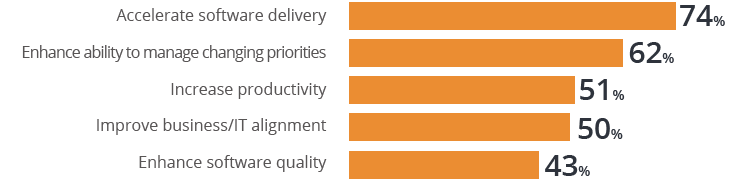
\includegraphics[width=.8\textwidth]{resources/Untitled}\\
		\caption{The Waterfall and Prototype SDLC models}
	\end{figure}

	Also the questionnaire contained a question about what are the recommended Agile project management tools.
	
	%todo modificare immagine
	\begin{figure}[H]
		\centering
		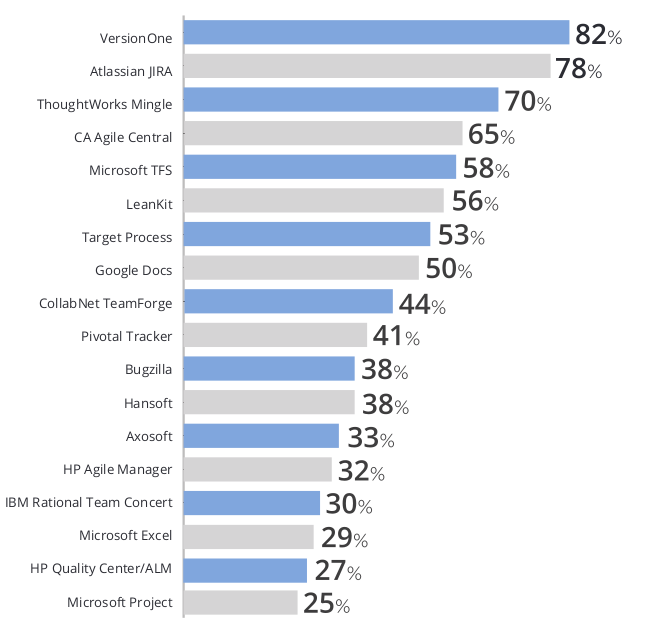
\includegraphics[width=.8\textwidth]{resources/Screenshot}\\
		\caption{The Waterfall and Prototype SDLC models}
	\end{figure}

	\begin{figure}[H]
		\centering
		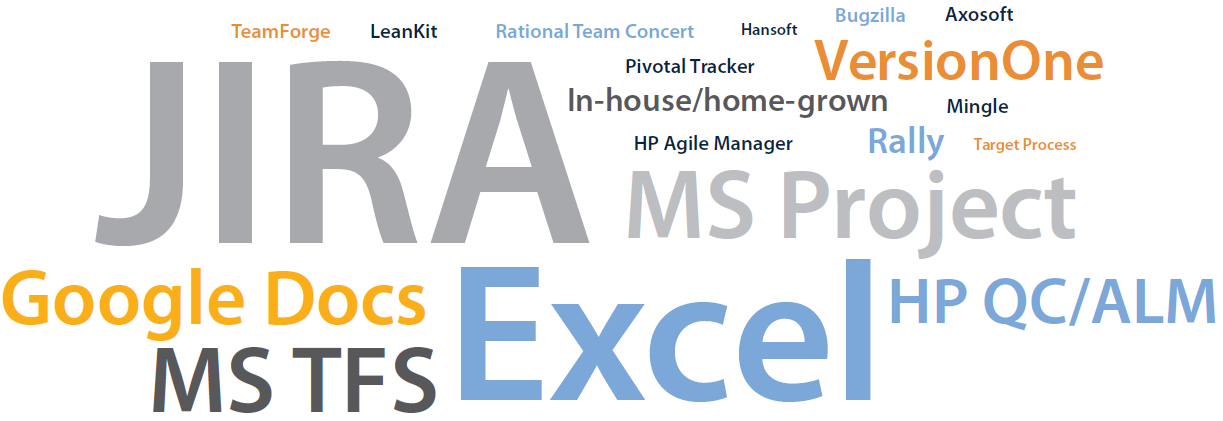
\includegraphics[width=.8\textwidth]{resources/Untitled_4}\\
		\caption{The Waterfall and Prototype SDLC models}
	\end{figure}

\section{Agile in practice}

% SPOTIFY
%https://medium.com/@media_75624/exploring-key-elements-of-spotifys-agile-scaling-model-471d2a23d7ea
%https://medium.com/productmanagement101/spotify-squad-framework-part-i-8f74bcfcd761

% AMAZON
%https://www.forbes.com/sites/stevedenning/2019/06/02/how-amazon-became-agile/

% MICROSOFT
%https://www.forbes.com/sites/stevedenning/2015/10/27/surprise-microsoft-is-agile/

% NETFLIX
%https://smartbear.com/blog/develop/5-lessons-agile-teams-can-learn-from-netflix/
%http://www.agileadvice.com/2018/03/02/profiles/a-case-study-of-netflixs-high-performance-culture/

LSD (Lean Software Development)
This methodology is an adaptation of the Toyota lean manufacturing principles to software development. It was introduced in 2009 by Marry and Tom Poppendieck in their book "Lean Software Development: An Agile Toolkit."


%https://www.inc.com/adam-fridman/the-massive-downside-of-agile-software-development.html
%https://leankit.com/learn/agile/what-are-the-disadvantages-of-agile/
\section{Disadvantages of Agile Software Development}
	l'agile può andare a completamente sostituire il resto\\
	cosa ne pensano gli utenti

\section{What Agile variant will Athonet use}
	misto a causa dei pochi dipendenti che hanno ancora una responsabilità ampia all'interno dell'azienda ma pensano che si possa incorporare agile\\
	processi di business

